For CSS hovedenheden er udviklet en række diagrammer ud fra applikationsmodel metoden.
Der er et sekvensdiagram på figur \ref{fig:CSS_hovedenhed_SD} for alle de aktuelle use-cases som beskriver systemets virkemåde.
Ud fra dette er der lavet et klassediagram på figur \ref{fig:CSS_hovedenhed_Class} som dækker de forskellige use-cases med controller klasser og kommunikationenen til PC via RS232 og X10 udtag via X10.


\begin{figure}[!htb]
	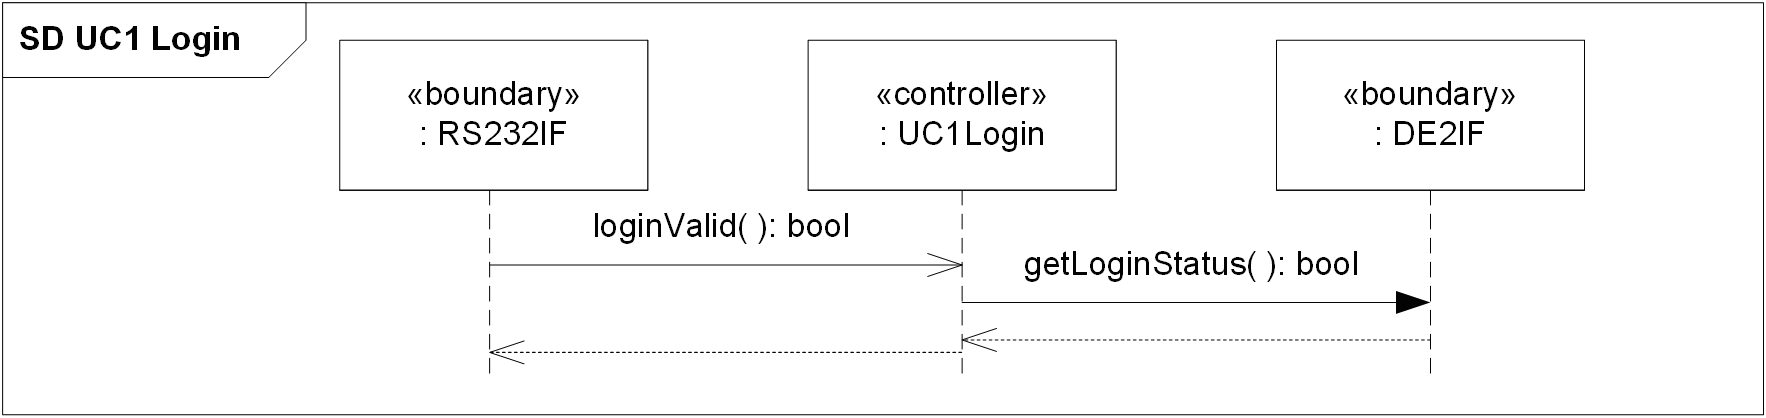
\includegraphics{billeder/uml/CSS_hovedenhed_SD}
     \caption{Use-case sekvensdiagrammer for CSS hovedenhed}
     \label{fig:CSS_hovedenhed_SD}
\end{figure}

\begin{figure}[!htb]
     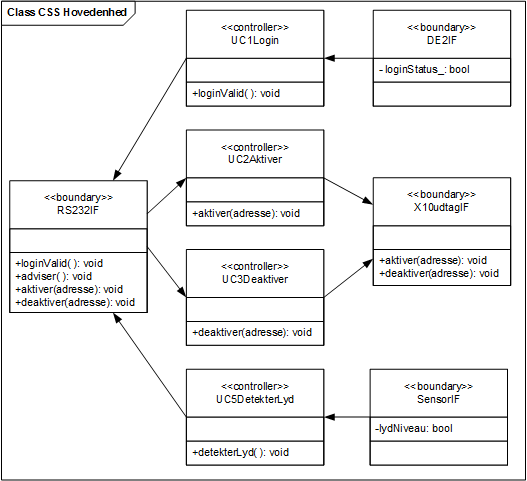
\includegraphics{billeder/uml/CSS_hovedenhed_Class}
     \caption{Klassediagram for CSS hovedenhed}
     \label{fig:CSS_hovedenhed_Class}
\end{figure}
